\documentclass{beamer}

\usetheme{Antibes}
\useoutertheme[subsection=false]{miniframes}

%\usetheme{split}
%\usetheme{Madrid}
%\usetheme{Berkeley}

\usecolortheme[RGB={120,0,0}]{structure}
\setbeamertemplate{blocks}[rounded][shadow=true]
\setbeamertemplate{footline}[frame number]
\setbeamersize{text margin left=.5cm,text margin right=.5cm} 
\usepackage[utf8]{inputenc}   % pacote para acentuao
\usepackage{graphicx}
\usepackage{subcaption}

%\usepackage[latin1]{inputenc}

\beamertemplateballitem
\beamertemplatenavigationsymbolsempty

\begin{document}

\title{Assessing the Computation and Communication Overhead of Linux Containers for HPC Applications}
\author{
\large 
\underline{Guilherme R. Alles}, Lucas M. Schnorr, Alexandre Carissimi\\
\small
\vspace*{0.5cm}
Instituto de Informática\\ Universidade Federal do Rio Grande do Sul \\\medskip

\includegraphics[width=.15\textwidth]{cnpq.png}%
\hspace{.5 cm}%
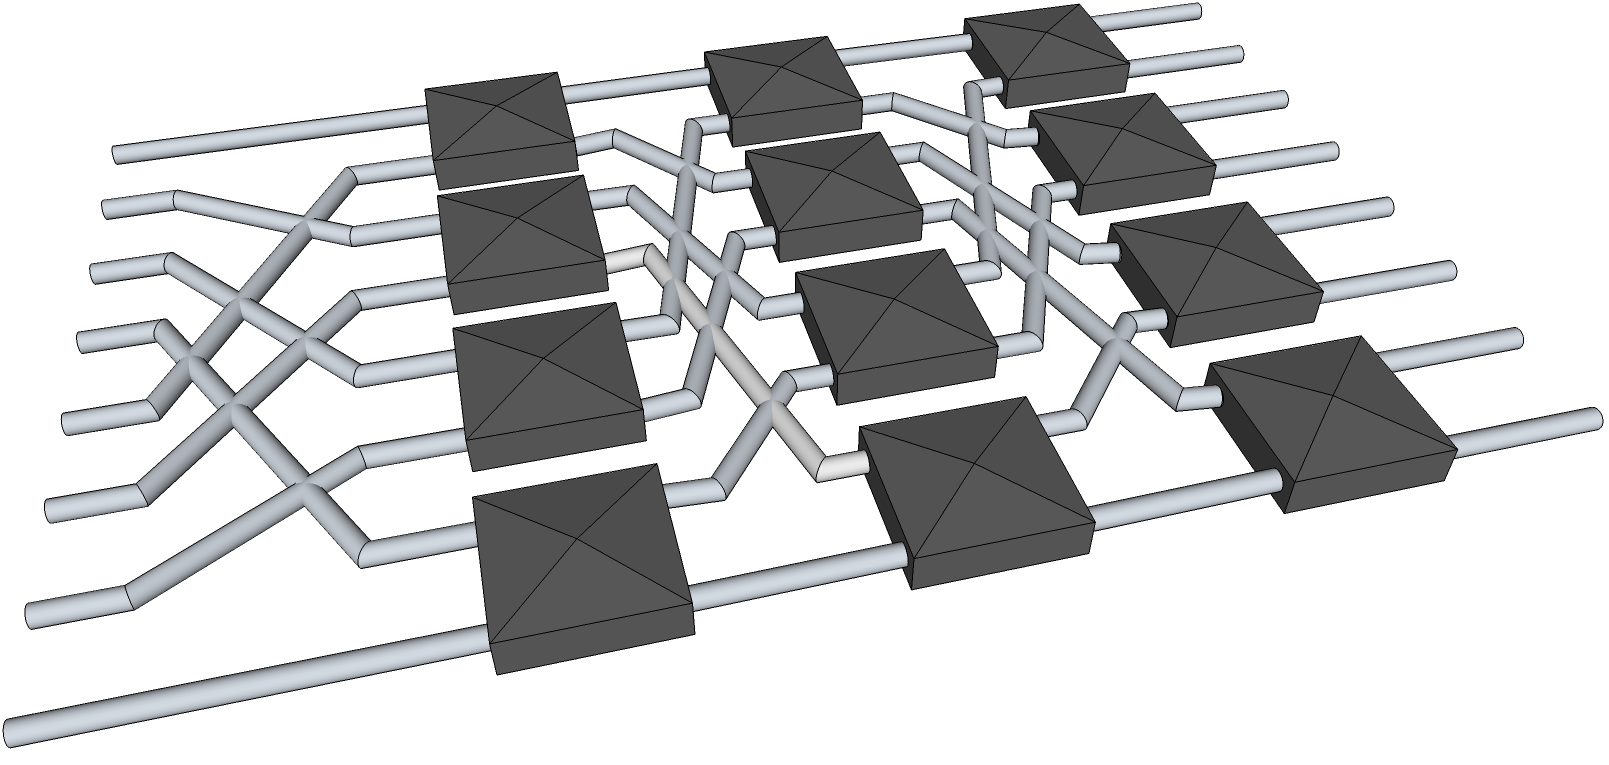
\includegraphics[width=.15\textwidth]{gppd-logo.png} \\\vspace{-.5cm}
}
\date{Simpósio de Sistemas Computacionais de Alto Desempenho\\
  2 de outubro de 2018}

\frame{\titlepage}

\section*{Introduction and Objectives}
\frame{\frametitle{Introduction}
        High-Performance Computing (HPC) clusters are \textbf{highly heterogeneous}
        \begin{itemize}
            \item Hardware configurations, software stacks, usage policies...
        \end{itemize}
        \pause
        \vspace*{0.3cm}
        Designing experiments for \underline{portability} requires investing time
        \begin{itemize}
            \item Operating system specifics
            \item Dependency management
        \end{itemize}
        \pause
        \vspace*{0.3cm}
        What if someone wants to \underline{reproduce} your experiments?
}

\frame{\frametitle{Introduction}
    Possible solution: virtual machines! \pause But...
    \begin{itemize}
        \item Requires a \textbf{hypervisor}. Which one?
        \begin{itemize}
            \item Type 1, Type 2, paravirtualization
            \item What if different clusters support different hypervisors?
        \end{itemize}
        \item Multi-gigabyte system images
        \item \textbf{Overhead}
    \end{itemize}
}

\frame{\frametitle{Introduction}
    Why can't we use Linux Containers?
    \begin{itemize}
        \pause
        \vspace*{0.2cm}
        \item No hypervisor overhead
        \pause
        \vspace*{0.2cm}
        \item Images take much less space
        \pause
        \vspace*{0.2cm}
        \item APIs integrated in the Linux Kernel
        \pause
        \vspace*{0.2cm}
        \item Flexibility yield performance gains at a small development cost
    \end{itemize}
}

\frame{\frametitle{Objectives}
        Measure \textbf{viability} of applying container technology to HPC
        \pause
        \begin{itemize}
            \item Computation overhead (application makespan)
            \item Communication overhead (latency/bandwidth)
        \end{itemize}
        \pause
        \vfill
        Contrast two popular container environments and their \textbf{workflows}
        \begin{itemize}
            \item Docker
            \item Singularity
        \end{itemize}
    \vfill
    {\hspace{2cm}
\includegraphics[width=.35\textwidth]{docker-logo.png}\hfill%

\includegraphics[width=.1\textwidth]{singularity-logo.png}\hspace{2cm}}
}

\frame{\frametitle{Outline}\tableofcontents[hideallsubsections]}

\section{Linux Containers}
\frame{\frametitle{Linux Containers}
  \vspace*{0.2cm}
  \centering
  \begin{columns}
    \begin{column}{0.5\textwidth}
      OS level virtualization

      \bigskip
      
      Build into the Linux Kernel
      \begin{itemize}
      \item \textbf{Resource control} (cgroups)
      \item \textbf{Isolation} (namespaces)
      \end{itemize}
    \end{column}
    \begin{column}{0.5\textwidth}
      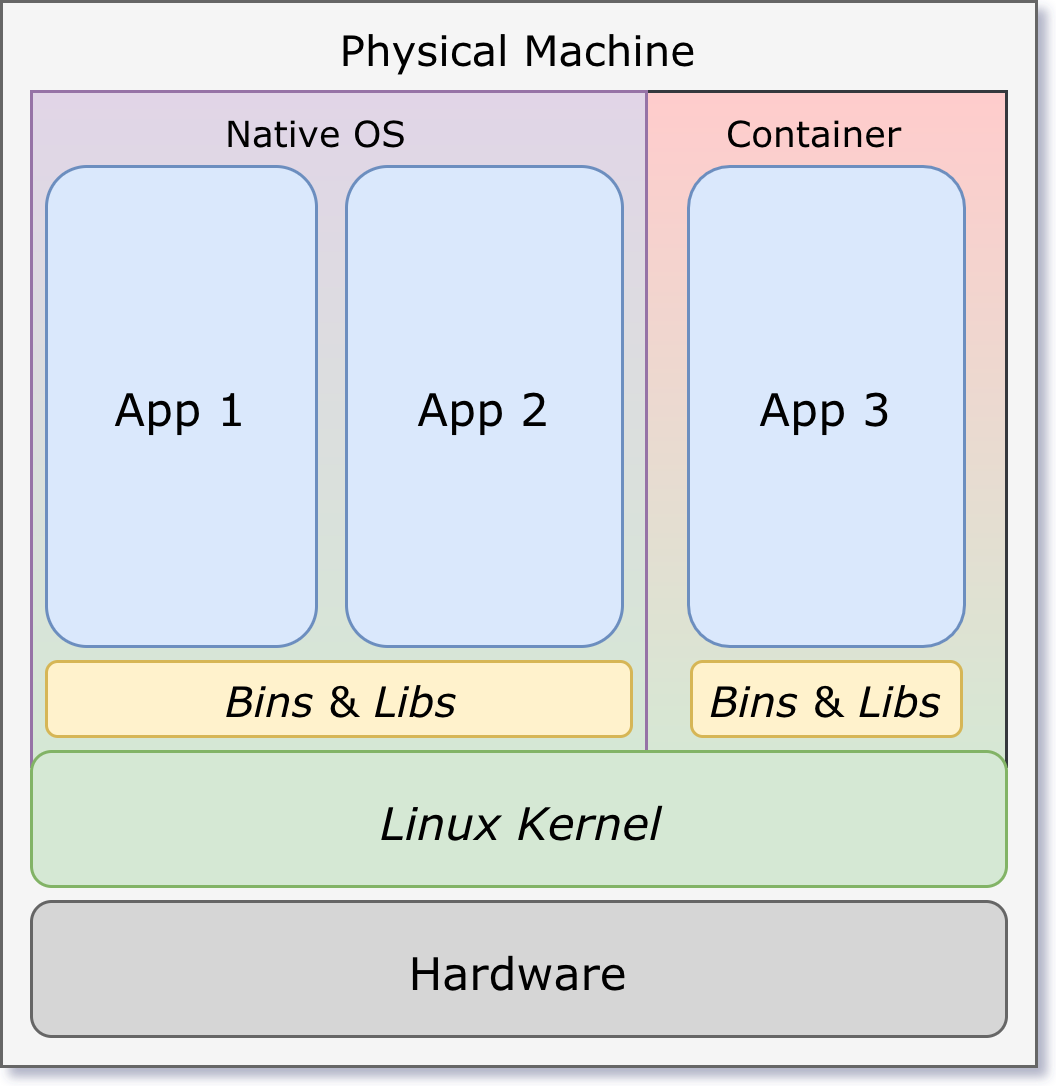
\includegraphics[width=\linewidth]{containers.png}
    \end{column}
  \end{columns}
}

\frame{\frametitle{Docker}
    \vspace*{-0.7cm}
    \begin{figure}
        \centering
        
\includegraphics[width=.5\textwidth]{docker-logo.png}
    \end{figure}
    \vspace*{-0.2cm}
    \begin{itemize}
    \item Widely used in the industry (for microservices virtualization)
    \item Standard in cloud IaaS providers such as AWS, GCP and Azure
      \pause\vfill
    \item Enforces virtualization for all six Linux Kernel namespace
      \begin{itemize}
      \item \emph{mount} (filesystem tree and mounts)
      \item \emph{PID} (process IDs)
      \item \emph{UTS} (host name and domain name)
      \item \emph{\bf network} (devices, ports, routing tables, firewall)
      \item \emph{IPC} (inter-process communication resources)
      \item \emph{\bf user} (unpriviliged, added in Linux 3.8)
      \end{itemize}
      \pause
    \item Implications on the use case (drawbacks for HPC)
    \end{itemize}
}

\frame{\frametitle{Singularity}
    \vspace*{-0.5cm}
    \begin{figure}
        \centering
        
\includegraphics[width=.2\textwidth]{singularity-logo.png}
    \end{figure}
    \vspace*{-0.2cm}
    \begin{itemize}
        \item Linux Containers for HPC
        \vspace*{0.2cm}
        \item Alternative to Docker drawbacks for shared environments
        \pause
        \vspace*{0.2cm}
        \item Objective: \textbf{secure} container environment for HPC clusters
        \pause
        \vspace*{0.2cm}
        \item Virtualizes \textbf{only the necessary
          namespaces} \\ Everything else is kept optional
        \begin{itemize}
            \item \textbf{file system}
        \end{itemize}
    \end{itemize}
}

\section{Experimental Design}
\frame{\tableofcontents[currentsection,hideothersubsections]}

\frame{\frametitle{Testbed}
  Grid5000's Graphene clusters (hardware)
  \begin{itemize}
  \item Intel Xeon X3340, 4 cores @ 2.53GHz
  \item 16GB DDR3 RAM
  \item Gigabit Ethernet interconnect
  \end{itemize}
  \pause
  \vfill
  Debian 9 (\textit{stretch}) Linux (software)
  \begin{itemize}
  \item Containers running on top of the native environment
  \item Docker containers connected through Docker Swarm \textit{overlay}
    \begin{itemize}
    \item Necessary because of \textbf{PID} and \textbf{network} virtualization
    \item Allows addressing MPI processes
    \end{itemize}
  \end{itemize}
}

\frame{\frametitle{Three Workloads}
    1. NAS Parallel Benchmarks
    \begin{itemize}
        \item Synthetic workload for baseline purposes
        \item EP (\textit{embarrassingly parallel}) Kernel
        \begin{itemize}
            \item CPU bound scenario
            \item Low communication between workers
            \item Workload size B
        \end{itemize}
    \end{itemize}
    \pause
    \vspace*{0.2cm}
    2. Ondes3D geophysics simulator (French BRGM)
    \begin{itemize}
        \item Seismic waves propagation simulation in heterogeneous media
        \item Spatial and temporal load imbalance, frequent communication
        \begin{itemize}
            \item Two inputs: simplified Chuetsu-Oki (test case) + Ligurian
        \end{itemize}
    \end{itemize}
    \vspace*{0.2cm}
    \pause
    3. Ad-hoc Ping-Pong benchmark
    \begin{itemize}
    \item Mostly focused on network latency \\
      $\to$ to verify how it would affect small messages
    \end{itemize}
}

\section{Results}
\frame{\tableofcontents[currentsection,hideothersubsections]}

\frame{\frametitle{Results -- NAS EP (Class B)}
  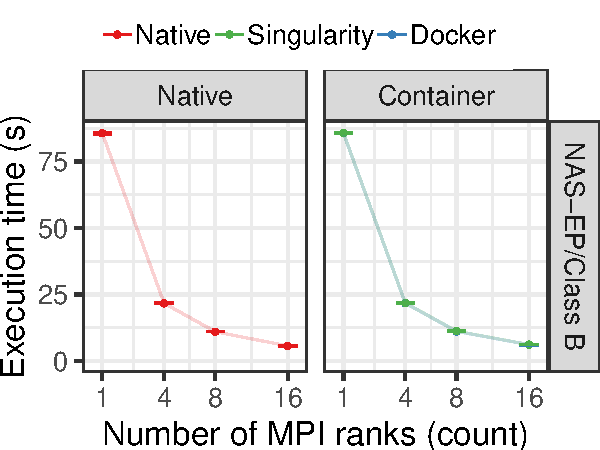
\includegraphics[width=.49\linewidth]{v2-nas-ep-raw.pdf}\hfill\pause%
  \only<3->{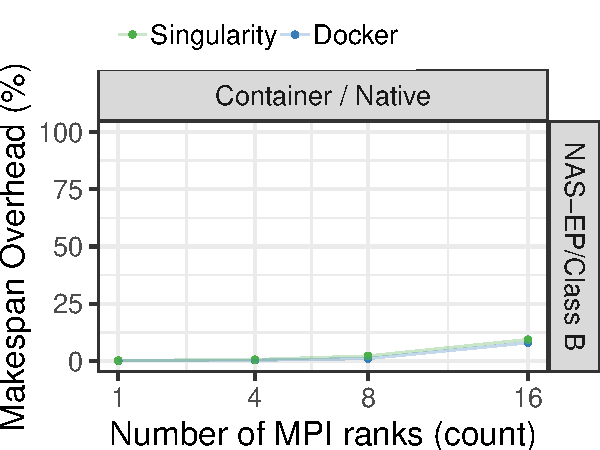
\includegraphics[width=.49\linewidth]{v2-nas-ep-overhead.pdf}}

  \vfill

  Observations

  \begin{itemize}
  \item Singularity and Docker are very similar to each other
  \item<3-> Overhead with 16 MPI ranks: Singularity ($\approx$9\%),
    Docker ($\approx$8\%) \\
  \item<4-> Overhead increases with the number of MPI ranks
  \end{itemize}
}

\frame{\frametitle{Results -- Ondes3D with simplified Chuetsu-Oki (small)}
  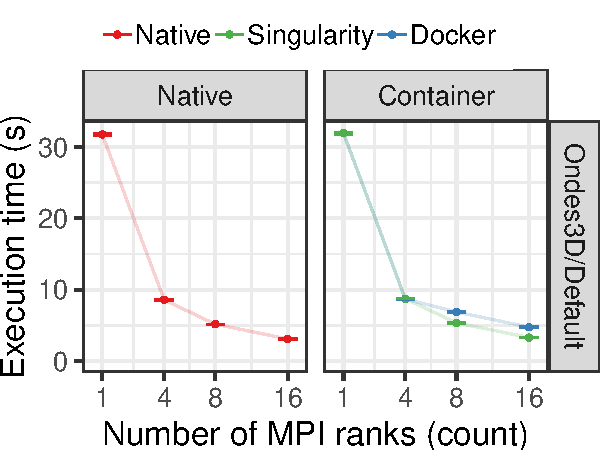
\includegraphics[width=.49\linewidth]{v2-ondes3d-default-raw.pdf}\hfill%
  \only<2->{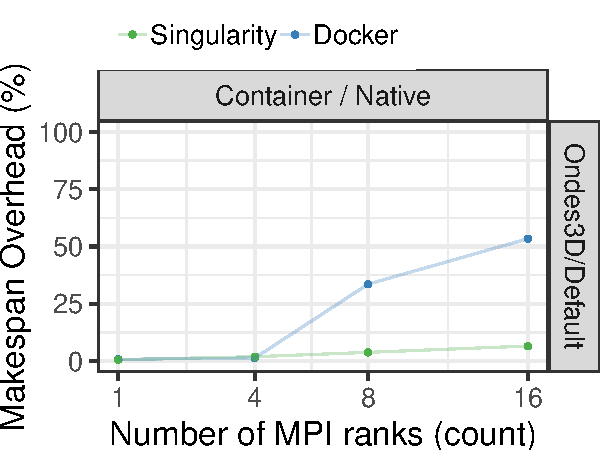
\includegraphics[width=.49\linewidth]{v2-ondes3d-default-overhead.pdf}}


  Observations

  \begin{itemize}
  \item Docker performance degrades when going up to 8 and 16 ranks
  \item<2-> Overhead of $\approx$33\% for 8 MPI ranks and
    $\approx$53\% for 16 \\
    More physical nodes $\to$ increase Docker swarm overhead
  \item<3-> Singularity has some overhead ($\approx$6\% for 16 ranks)  \\
    $\to$ For same reasons of compute-bound NAS EP (previous slide)
  \end{itemize}
}

\frame{\frametitle{Results -- Ondes3D with Ligurian (large)}

Only with Singularity due to Docker swarm communication overhead
  
    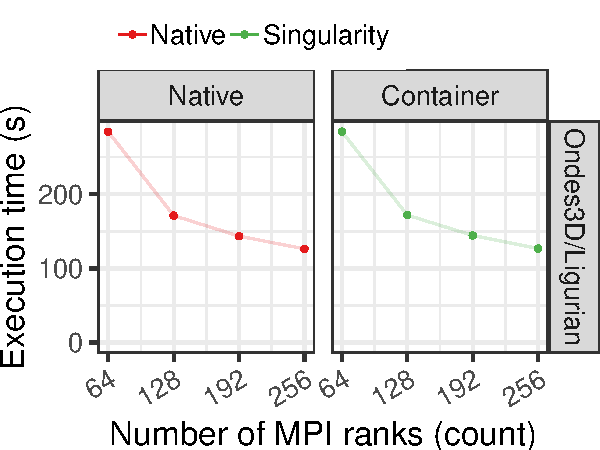
\includegraphics[width=.49\linewidth]{v2-ondes3d-ligurian-raw.pdf}\hfill\pause%
    \only<3->{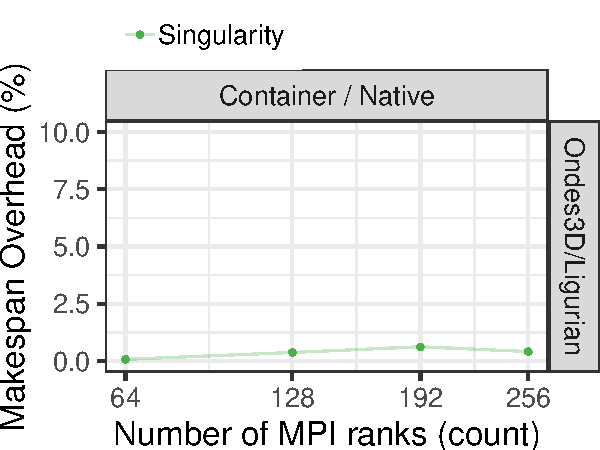
\includegraphics[width=.49\linewidth]{v2-ondes3d-ligurian-overhead.pdf}}

  Observations

  \begin{itemize}
  \item No observable difference in execution time
  \item<3-> Minor overhead of less than $\approx$1\% in all cases \\
    $\to$ Container initialization time gets absorbed
  \item<4-> Overhead is smaller with 256 ranks     $\to$ Smaller returns on speedup
  \end{itemize}
}

\frame{\frametitle{Results -- Ping Pong (measuring network latency)}
  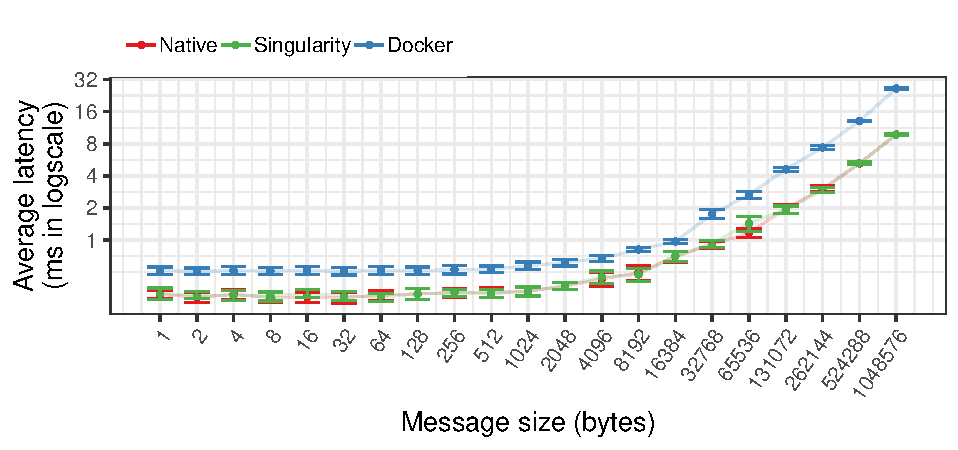
\includegraphics[width=\linewidth]{v2-network-latency-raw.pdf}

  \vfill\pause
  
  \begin{itemize}
  \item Docker network latency is much higher \\
    $\to$ As previous experiments have shown
  \item\pause Singularity containers use the native network stack \\
    $\to$ Non-observable performance differences
  \end{itemize}
}

\frame{\frametitle{Results -- Optimized Container based on Alpine Linux}
  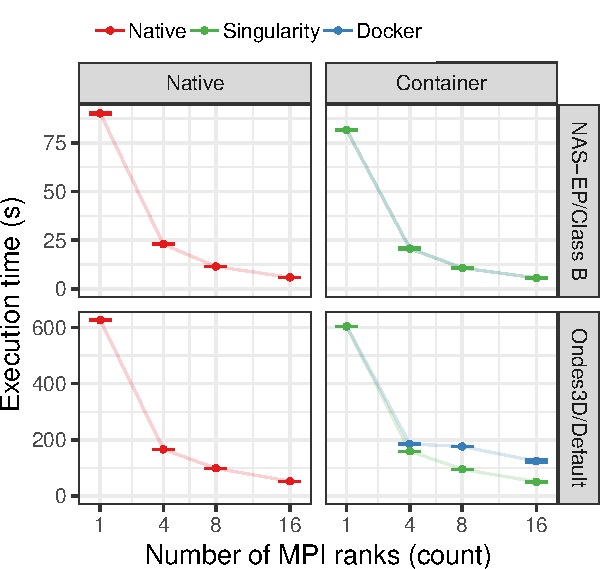
\includegraphics[width=.53\linewidth]{v2-alpine-nas-ondes3d-raw.pdf}\hfill\pause%
  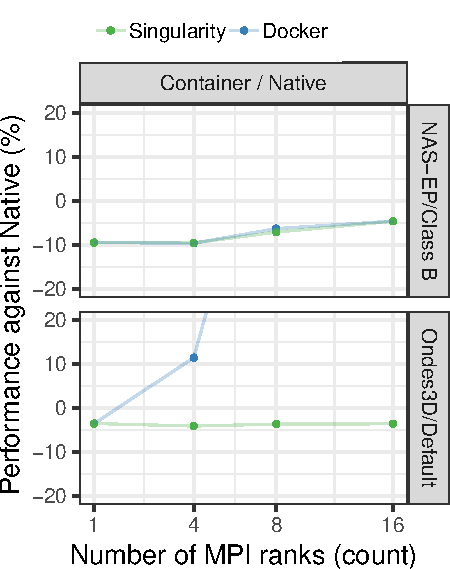
\includegraphics[width=.39\linewidth]{v2-alpine-nas-ondes3d-overhead.pdf}

  Observations
  \begin{itemize}
  \item Virtualized execution to outperform the native one
  \item Singularity/Alpine is $\approx$5\% on the Ondes3D/Default case 
  \end{itemize}
}

\section{Conclusions and Future Work}
\frame{\tableofcontents[currentsection,hideothersubsections]}

\frame{\frametitle{Conclusions}
    \begin{itemize}
        \item Containers are a viable way of virtualizing an HPC environment
        \pause
        \item Computational overhead is negligible in most use cases
        \pause
        \item Communication overhead is significant, especially with Docker
        \begin{itemize}
            \item Virtualization of the \textbf{network} namespace impacts MPI workloads
        \end{itemize}
        \pause
        \item Performance gains are attainable by \textbf{fine tuning} the environment
    \end{itemize}
}

\frame{\frametitle{Future Work}
  Further investigate Docker Swarm scalability
    \begin{itemize}
    \item Increased latency
    \item Failure to spawn a larger number of containers
    \end{itemize}
    \pause\vfill    
  Explore container compatibility with other devices
    \begin{itemize}
    \item GPU
    \item InfiniBand
    \end{itemize}
    \pause\vfill    
 Evaluate CharlieCloud: follows the UNIX philosophy \\
    
\includegraphics[width=.25\textwidth]{charliecloud.png}%        
}

\frame{\frametitle{Thank you for your attention! Questions?}

  Some experiments have been conducted in the Grid5000 platform
  \begin{itemize}
  \item \url{https://www.grid5000.fr}
  \end{itemize}

  Investigation based on a reproducible workflow, source code and data
  \begin{itemize}
  \item \url{https://github.com/guilhermealles/hpc-containers/}
  \end{itemize}

  \vfill

  \centering Contact with Guilherme Rezende Alles

  \centering\url{gralles@inf.ufrgs.br}

  \vfill

  \hfill\scalebox{0.5}{

    \begin{minipage}{\textwidth}
      {\bf     Acknowledgments:} We thank these projects for supporting this investigation:
      FAPERGS GreenCloud (16/488-9), the FAPERGS MultiGPU (16/354-8),
      the CNPq 447311/2014-0, the CAPES/Brafitec EcoSud 182/15, and
      the CAPES/Cofecub 899/18. Experiments were carried out at the
      Grid'5000 platform ({\texttt{https://www.grid5000.fr}}), with
      support from Inria, CNRS, RENATER and several other french
      organizations. The companion material is hosted by GitHub for
      which we are also grateful.
    \end{minipage}
  }

}

\end{document}
